\documentclass[12pt]{article}
\usepackage{amsmath}
\usepackage{graphicx}
\usepackage{hyperref}
\usepackage{listings}
\usepackage{color}
\usepackage{pythonhighlight}

\title{Operating System Course Report - First Half of the Semester}
\author{B class}
\date{\today}

\begin{document}

\maketitle
\newpage

\tableofcontents
\newpage

\section{Introduction}
This report summarizes the topics covered during the first half of the
Operating System course. It includes theoretical concepts, practical
implementations, and assignments. The course focuses on the fundamentals of
operating systems, including system architecture, process management, CPU
scheduling, and deadlock handling.

\section{Course Overview}
\subsection{Objectives}
The main objectives of this course are:
\begin{itemize}
    \item To understand the basic components and architecture of a computer system.
    \item To learn process management, scheduling, and inter-process communication.
    \item To explore file systems, input/output management, and virtualization.
    \item To study the prevention and handling of deadlocks in operating systems.
\end{itemize}

\subsection{Course Structure}
The course is divided into two halves. This report focuses on the first half,
which covers:
\begin{itemize}
    \item Basic Concepts and Components of Computer Systems
    \item System Performance and Metrics
    \item System Architecture of Computer Systems
    \item Process Description and Control
    \item Scheduling Algorithms
    \item Process Creation and Termination
    \item Introduction to Threads
    \item File Systems
    \item Input and Output Management
    \item Deadlock Introduction and Prevention
    \item User Interface Management
    \item Virtualization in Operating Systems
\end{itemize}

\section{Topics Covered}

\subsection{Basic Concepts and Components of Computer Systems}
This section explains the fundamental components that make up a computer
system, including the CPU, memory, storage, and input/output devices.

\subsection{System Performance and Metrics}
This section introduces various system performance metrics used to measure the
efficiency of a computer system, including throughput, response time, and
utilization.

\subsection{System Architecture of Computer Systems}
Describes the architecture of modern computer systems, focusing on the
interaction between hardware and the operating system.

\subsection{Process Description and Control}
Processes are a central concept in operating systems. This section covers:
\begin{itemize}
    \item Process states and state transitions
    \item Process control block (PCB)
    \item Context switching
\end{itemize}

\subsection{Scheduling Algorithms}
This section covers:
\begin{itemize}
    \item First-Come, First-Served (FCFS)
    \item Shortest Job Next (SJN)
    \item Round Robin (RR)
\end{itemize}
It explains how these algorithms are used to allocate CPU time to processes.

\subsection{Process Creation and Termination}
Details how processes are created and terminated by the operating system,
including:
\begin{itemize}
    \item Process spawning
    \item Process termination conditions
\end{itemize}

\subsection{Introduction to Threads}
This section introduces the concept of threads and their relation to processes,
covering:
\begin{itemize}
    \item Single-threaded vs. multi-threaded processes
    \item Benefits of multithreading
\end{itemize}

% \begin{figure}[h]
%     \centering
%     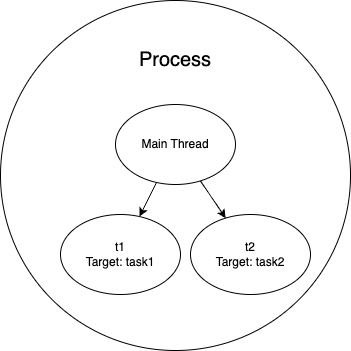
\includegraphics[width=0.5\textwidth]{./b_class/asset/example.png}  % Sesuaikan nama file dan ukurannya
%     \caption{Ini adalah gambar contoh dari multithreading.}
%     \label{fig:contoh_gambar}
% \end{figure}

Seperti yang terlihat pada Gambar \ref{fig:contoh_gambar}, inilah cara
menambahkan gambar dengan keterangan.

\subsection{File Systems}
File systems provide a way for the operating system to store, retrieve, and
manage data. This section explains:
\begin{itemize}
    \item File system structure
    \item File access methods
    \item Directory management
\end{itemize}

\subsection{Input and Output Management}
Input and output management is key for handling the interaction between the
system and external devices. This section includes:
\begin{itemize}
    \item Device drivers
    \item I/O scheduling
\end{itemize}

\subsection{Deadlock Introduction and Prevention}
Explores the concept of deadlocks and methods for preventing them:
\begin{itemize}
    \item Deadlock conditions
\end{itemize}
\subsubsection{Kelebihan dan Kekurangan Deadlock prevention}

\hspace{1cm} Pencegahan terhadap deadlock adalah teknik yang digunakan untuk mencegah sistem memasuki keadaan deadlock.
Berbeda dengan deadlock avoidance yang dimana mengatasi masalah setelah deadlock terjadi, pencegahan ada agar memperkecil
kemungkinan terjadinya deadlock. Pencegahan deadlock dapat dilakukan dengan cara menghindari keadaan-keadaan yang dapat menyebabkan deadlock.
Beberapa kelebihan dan kekurangan metode pencegahan deadlock adalah:

\begin{enumerate}
    \item Resources Ordering

            \hspace{0cm} Kelebihan:
            \begin{itemize}
              \item Mencegah circular wait
              \item Sederhana untuk diterapkan
              \item Mencegah deadlock secara proaktif
            \end{itemize}


            \hspace{0cm} Kekurangan:
            \begin{itemize}
              \item Kurangnya fleksibilitas
              \item Kompleksitas pada sistem besar
              \item Overhead pengelolaan
            \end{itemize}

          \hspace{1cm}Resource Ordering cocok untuk sistem kecil dan statis karena mudah dikelola, tetapi menjadi terlalu rumit pada sistem besar dengan banyak sumber daya.

    \item Resource allocation denial

          \hspace{0cm} Kelebihan:
            \begin{itemize}
              \item Sederhana dan efektif
              \item Mencegah deadlock secara langsung
            \end{itemize}


            \hspace{0cm} Kekurangan:
            \begin{itemize}
              \item Penggunaan sumber daya yang tidak efisien
              \item Keterbatasan dalam fleksibilitas sistem
            \end{itemize}

        \hspace{1cm}Resource Allocation Denial cocok untuk sistem kritis yang membutuhkan kontrol ketat atas penggunaan sumber daya, tetapi bisa mengurangi efisiensi.

    \item Timeouts

          \hspace{0cm} Kelebihan:
            \begin{itemize}
              \item Sederhana untuk diimplementasikan
              \item Mencegah deadlock dengan menghentikan proses
            \end{itemize}


            \hspace{0cm} Kekurangan:
            \begin{itemize}
              \item Risiko palsu positif
              \item Overhead sistem dari manajemen timeout
            \end{itemize}

          \hspace{1cm}Timeouts ideal untuk lingkungan I/O yang intensif di mana operasi berjangka panjang dapat mengalami deadlock jika tidak dikelola dengan tepat.

    \item Avoidance of hold-and-wait conditions

          \hspace{0cm} Kelebihan:
            \begin{itemize}
              \item Mencegah deadlock secara efektif
              \item Mengurangi risiko deadlock
            \end{itemize}


            \hspace{0cm} Kekurangan:
            \begin{itemize}
              \item Penggunaan sumber daya kurang efisien
              \item Overhead administratif
            \end{itemize}

          \hspace{1cm}Avoidance of Hold-and-Wait baik untuk proses jangka panjang atau batch yang memerlukan banyak sumber daya, namun kurang efisien dalam alokasi sumber daya.
    \item Resource preemption

          \hspace{0cm} Kelebihan:
            \begin{itemize}
              \item Efektif dalam mengatasi deadlock
              \item Fleksibel untuk sistem yang berjalan
            \end{itemize}


            \hspace{0cm} Kekurangan:
            \begin{itemize}
              \item Overhead dan biaya
              \item Kehilangan proses dan potensi kehilangan data
            \end{itemize}

          \hspace{1cm}Resource Preemption cocok untuk sistem multitasking dengan banyak sumber daya yang dapat dipreempt, tetapi harus berhati-hati terhadap kehilangan data.
\end{enumerate}

\subsection{User Interface Management}
This section discusses the role of the operating system in managing the user
interface. Topics covered include:
\begin{itemize}
    \item Graphical User Interface (GUI)
    \item Command-Line Interface (CLI)
    \item Interaction between the user and the operating system
\end{itemize}

\subsection{Virtualization in Operating Systems}
Virtualization allows multiple operating systems to run concurrently on a
single physical machine. This section explores:
\begin{itemize}
    \item Concept of virtualization
    \item Hypervisors and their types
    \item Benefits of virtualization in modern computing
\end{itemize}

\section{Assignments and Practical Work}
\subsection{Assignment 1: Process Scheduling}
Students were tasked with implementing various process scheduling algorithms
(e.g., FCFS, SJN, and RR) and comparing their performance under different
conditions.
\subsubsection{Group 1}
\begin{python}
    class Process:
    def _init_(self, pid, arrival_time, burst_time):
    self.pid = pid
    self.arrival_time = arrival_time
    self.burst_time = burst_time
    self.completion_time = 0
    self.turnaround_time = 0
    self.waiting_time = 0
\end{python}

\begin{table}[htbp] % Optional: For floating position
    \centering
    \begin{tabular}{|c|c|c|} % Defines number of columns and alignment (c = center, l = left, r = right). '|' creates vertical lines.
        \hline
        Header 1        & Header 2        & Header 3        \\ % Column headers
        \hline
        Row 1, Column 1 & Row 1, Column 2 & Row 1, Column 3 \\ % First row of data
        \hline
        Row 2, Column 1 & Row 2, Column 2 & Row 2, Column 3 \\ % Second row of data
        \hline
    \end{tabular}
    \caption{Your table caption} % Optional: For adding a caption
    \label{tab:your_label} % Optional: For cross-referencing the table
\end{table}

\subsection{Assignment 2: Deadlock Handling}
In this assignment, students were asked to simulate different deadlock
scenarios and explore various prevention methods.

\subsection{Assignment 3: Multithreading and Amdahl's Law}
This assignment involved designing a multithreading scenario to solve a
computationally intensive problem. Students then applied *Amdahl's Law* to
calculate the theoretical speedup of the program as the number of threads
increased.
\subsubsection{Kelompok 11}
\subsubsection*{Soal : }
Buatkan sebuah program \texttt{Python} yang menggunakan \textbf{multithreading} untuk menyelesaikan masalah komputasi intensif berupa perhitungan jumlah bilangan prima dalam suatu rentang bilangan. Setelah itu, terapkan \textbf{Amdahl's Law} untuk menghitung \textit{speedup} teoritis dari program ketika jumlah thread ditingkatkan.\\
\\

\subsection*{Jawaban}
\begin{enumerate}
    \item \textbf{Implementasi Multithreading}:
    \begin{itemize}
        \item Buatlah program yang menghitung jumlah bilangan prima dalam rentang bilangan dari 1 hingga 500.000 menggunakan \textbf{multithreading}.
        \item Anda harus mengimplementasikan program dengan 1, 2, 4, dan 8 thread untuk membandingkan waktu eksekusi.
    \end{itemize}

    \item \textbf{Amdahl's Law}:
    \begin{itemize}
        \item Misalkan 20\% dari program tidak bisa diparalelkan (bersifat serial).
        \item Gunakan rumus \textbf{Amdahl's Law} berikut untuk menghitung \textit{speedup} teoritis berdasarkan jumlah thread (\(N\)):
        \[
        S(N) = \frac{1}{(1 - P) + \frac{P}{N}}
        \]
        Di mana:
        \begin{itemize}
            \item \(P = 0.8\) adalah proporsi kode yang bisa diparalelkan (80\%).
            \item \(N\) adalah jumlah thread (1, 2, 4, 8).
        \end{itemize}
    \end{itemize}

    \begin{python}
        import threading
import time

# Fungsi untuk memeriksa apakah sebuah bilangan prima
def is_prime(n):
    if n < 2:
        return False
    for i in range(2, int(n**0.5) + 1):
        if n % i == 0:
            return False
    return True

# Fungsi untuk menghitung bilangan prima dalam rentang tertentu
def count_primes(start, end, result, index):
    count = 0
    for num in range(start, end):
        if is_prime(num):
            count += 1
    result[index] = count

# Fungsi untuk menjalankan perhitungan dengan multithreading
def prime_counter_with_threads(range_start, range_end, num_threads):
    threads = []
    result = [0] * num_threads
    segment_size = (range_end - range_start) // num_threads

    for i in range(num_threads):
        start = range_start + i * segment_size
        end = start + segment_size if i != num_threads - 1 else range_end
        t = threading.Thread(target=count_primes, args=(start, end, result, i))
        threads.append(t)
        t.start()

    for t in threads:
        t.join()

    return sum(result)

# Fungsi untuk menghitung waktu eksekusi
def test_prime_counter(range_start, range_end, num_threads):
    start_time = time.time()
    prime_count = prime_counter_with_threads(range_start, range_end, num_threads)
    end_time = time.time()
    execution_time = end_time - start_time
    print(f"Threads: {num_threads}, Waktu: {execution_time:.4f} detik, Bilangan Prima Ditemukan: {prime_count}")
    return execution_time

# Fungsi untuk menghitung speedup berdasarkan Amdahl's Law
def amdahls_law(P, N):
    return 1 / ((1 - P) + (P / N))

# Main program untuk melakukan pengujian
def main():
    range_start = 1
    range_end = 500000
    serial_fraction = 0.2  # 20% dari kode adalah serial
    parallel_fraction = 1 - serial_fraction  # 80% adalah paralel

    # Menguji dengan berbagai jumlah thread
    thread_counts = [1, 2, 4, 8]
    execution_times = []

    print("Menghitung bilangan prima dan mengukur waktu eksekusi:")
    for num_threads in thread_counts:
        execution_time = test_prime_counter(range_start, range_end, num_threads)
        execution_times.append(execution_time)

    print("\nMenghitung speedup teoritis berdasarkan Amdahl's Law:")
    for num_threads in thread_counts:
        theoretical_speedup = amdahls_law(parallel_fraction, num_threads)
        print(f"Threads: {num_threads}, Speedup Teoritis: {theoretical_speedup:.4f}")

    print("\nMembandingkan hasil eksekusi dan speedup teoritis:")
    base_time = execution_times[0]  # Waktu eksekusi dengan 1 thread sebagai baseline
    for i, num_threads in enumerate(thread_counts):
        actual_speedup = base_time / execution_times[i]
        theoretical_speedup = amdahls_law(parallel_fraction, num_threads)
        print(f"Threads: {num_threads}, Speedup Aktual: {actual_speedup:.4f}, Speedup Teoritis: {theoretical_speedup:.4f}")

if __name__ == "__main__":
    main()

    \end{python}


\subsubsection*{Waktu Eksekusi dan Jumlah Bilangan Prima yang Ditemukan:}
\begin{itemize}
    \item \textbf{Threads: 1}, Waktu: 0.2519 detik, Bilangan Prima Ditemukan: 9592
    \item \textbf{Threads: 2}, Waktu: 0.2355 detik, Bilangan Prima Ditemukan: 9592
    \item \textbf{Threads: 4}, Waktu: 0.2352 detik, Bilangan Prima Ditemukan: 9592
    \item \textbf{Threads: 8}, Waktu: 0.2536 detik, Bilangan Prima Ditemukan: 9592
\end{itemize}

\subsubsection*{Speedup Teoritis Berdasarkan Amdahl's Law:}
\begin{itemize}
    \item \textbf{Threads: 1}, Speedup Teoritis: 1.0000
    \item \textbf{Threads: 2}, Speedup Teoritis: 1.6667
    \item \textbf{Threads: 4}, Speedup Teoritis: 2.5000
    \item \textbf{Threads: 8}, Speedup Teoritis: 3.3333
\end{itemize}



\subsection{Assignment 4: Simple Command-Line Interface (CLI) for User Interface Management}
Students were tasked with creating a simple *CLI* for user interface
management. The CLI should support basic commands such as file manipulation
(creating, listing, and deleting files), process management, and system status
reporting.

\subsection{Assignment 5: File System Access}
In this assignment, students implemented file system access routines,
including:
\begin{itemize}
    \item File creation and deletion
    \item Reading from and writing to files
    \item Navigating directories and managing file permissions
\end{itemize}

\section{Conclusion}
The first half of the course introduced core operating system concepts,
including process management, scheduling, multithreading, and file system
access. These topics provided a foundation for more advanced topics to be
covered in the second half of the course.

\end{document}